\subsection*{1.9.1 Team Organization}
\addcontentsline{toc}{subsection}{1.9.1 Team Organization}

\begin{figure}[H]
    \centering
    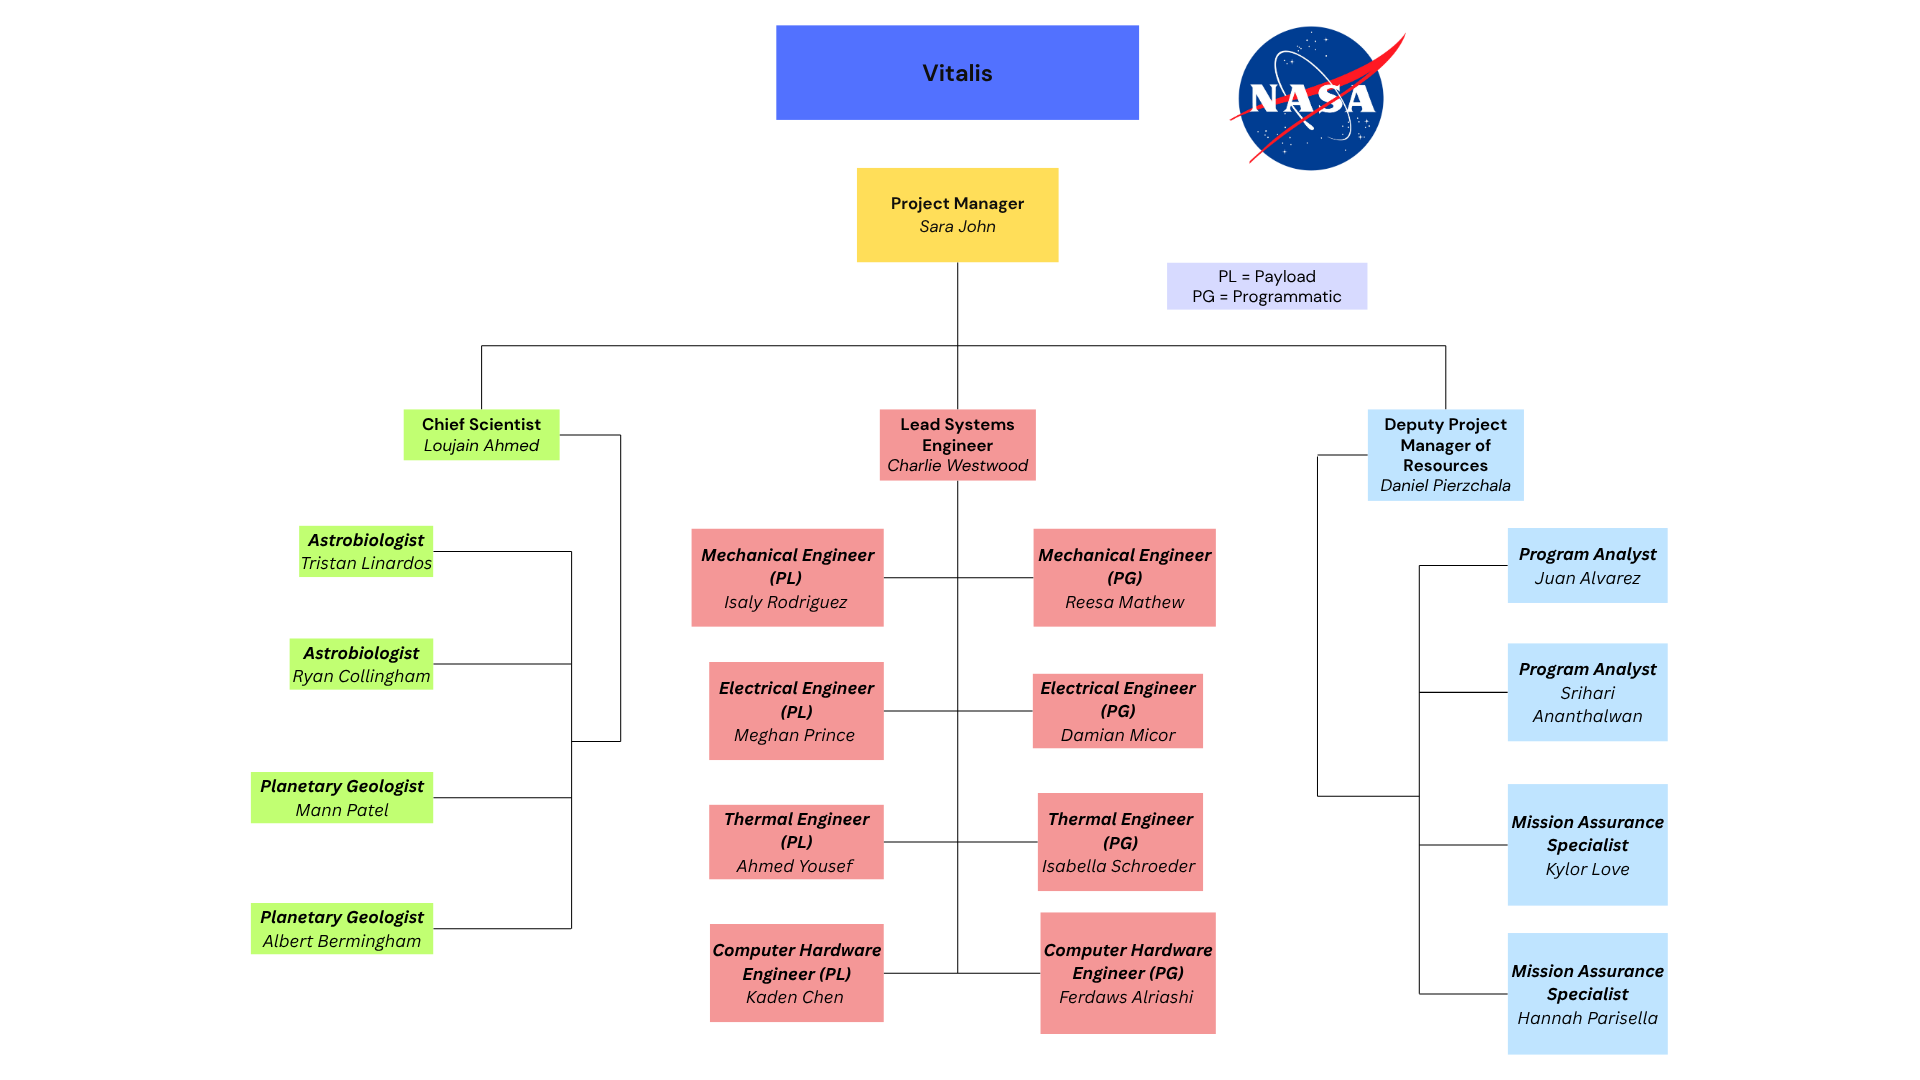
\includegraphics[width=1\textwidth]{images/orgchart.png}
    \caption{Team Organization Chart}
    \label{fig:orgchart}
\end{figure}

The organization of a team is essential to effectively tackling challenges and deliverables. Factors of success which will lead this team towards the completion of their mission come from the choices made in decision making and problem-solving methodologies, the process of workload delegation, and organization structure.

Allocating tasks will be determined by categorizing the task as belonging to a particular sub-team and role. From there, it will be up to the individuals within that role to volunteer themselves based on their self-perceived capabilities. This allows the most confident and qualified individuals to accomplish components of the mission quickly.

To help resolve some of the inevitable obstacles this mission will bring, the team will utilize varying methodologies depending on the technicality of the issue and allowable time. For technical issues, trade studies will be used to grade the solutions and system under criteria related to the mission to reveal which is optimal. For decisions which are time-sensitive or in an area which is not technical, those will be handled democratically. This style has the strength of allowing anyone to take the floor and present their ideas. This welcomes members of a different specialty to provide out-of-the-box thinking to create unique answers to potential problems. These ideas are voted upon with a majority choosing how to move forward. A democratic vote ensures participation from everyone, hence giving all a sense of ownership in decision.

The likelihood of success in this endeavor is too early to be certain. As in these beginning stages all members are getting acquainted with their roles and responsibilities. The dynamics that this mission and their team are relatively unknown. Yet these shortcomings are only temporary as greater utilization of communication skills and resources are improving the team’s ability to meet deliverables daily. Many within the team plan to train with the skill modules, attend all related meetings, and read the handbooks offered. Once these habits are integrated with the team’s developing schedule system, success is assured.

\begin{table}[H]
\centering
\caption{Team’s Weekly Availability}
\label{tab:availability}
\begin{tabular}{|>{\raggedright}p{4cm}|>{\raggedright}p{6cm}|c|}
\hline
\textbf{Name} & \textbf{Role} & \textbf{Availability (hrs/week)} \\
\hline
Sara John & Project Manager & 8--10 \\
Daniel Pierzchala & Deputy Project Manager of Resources & 8--10 \\
Loujan Ahmed & Chief Scientist & 8--10 \\
Charlie Westwood & Lead Systems Engineer & 8--10 \\
Tristan Linardos & Astrobiologist & 4--6 \\
Ryan Collingham & Astrobiologist & 8--10 \\
Mann Patel & Planetary Geologist & 8--10 \\
Albert Bermingham & Planetary Geologist & 8--10 \\
Isaly Rodriguez & Mechanical Engineer (Payload) & 10+ \\
Meghan Prince & Electrical Engineer (Payload) & 6--8 \\
Ahmed Yousef & Thermal Engineer (Payload) & 8--10 \\
Kaden Chen & Computer Hardware Engineer (Payload) & 6--8 \\
Reesa Mathew & Mechanical Engineer (Programmatics) & 6--8 \\
Damian Micor & Electrical Engineer (Programmatics) & 4--6 \\
Isabella Schroeder & Thermal Engineer (Programmatics) & 8--10 \\
Ferdaws Alriashi & Computer Hardware Engineer (Programmatics) & 10+ \\
Juan Alvarez & Program Analyst & 8--10 \\
Srihari Ananthalwan & Program Analyst & 8--10 \\
Kylor Love & Mission Assurance Specialist & 6--8 \\
Hannah Parisella & Mission Assurance Specialist & 10+ \\
\hline
\end{tabular}
\end{table}